This sections will cover necessary background information related to this thesis. It will summaries the most important features of the Encore Language such as Active objects, futures and the type system.

\section{Encore}
Encore is developed at the Programming Languages Group \citep{researchgroup} at Uppsala University and it is founded by the European project Upscale \citep{upscale}. Encore has been in development since 2014 and is planed to be open sourced released during the summer 2017. \\

Encore is a typed high-level object oriented programming language with many functional features, it focus on parallelism and achieves it by using the actor model. Every Encore program has at least one actor but Encore has support for millions of actors even on a machine with only has a few cores. \\

Encores compiler is written in Haskell \citep{website:haskell} and it translates Encore code to C code which later can be compiled with a C compiler. The Encore philosophy: \\ \\ \say{Encore is an actor-based parallel programming language aimed at general purpose parallel programming. By adopting the actor concurrency model, Encore avoids scalability problems associated with multi-threading. Encore offers an array of concurrency and parallelism abstractions beyond the pure actor model. These abstractions use Encore's capability type system to ensure that no data races occur.} \citep{encore}

\subsection{Active-Objects}
In Encore both passive and active classes exists. If you declarer an active class in Encore all method calls are asynchronous and methods are called with the bang operator (!) instead of with the dot as for normal classes. Each active-object has it’s own message queue and process each message sequentially, every active-object is one actor. Sense actors don’t share any memory with each other and with restriction on how objects are shared \citep{kappa} in Encore there can be no data-races. The big benefit of active-objects is that they can be scheduled on different cores without the programmers involvement, on negative side there are an overhead when using message sending instead of normal method calls \citep{encore_paper}. The Active-Objects embrace the actor model but also provide programs to be written in an object oriented fashion.

\subsection{Futures}
Futures is an important building block of Encore. In Encore and the active-object model there are a lot of message sending between active-objects. Messages may return futures. A future is a placeholder for a value that is returned from an asynchronous call. The Future is returned immediately to the callee but the return value can be stored later during the programs execution. Reading a value before the futures has been fulfilled will result in blocking state where the reader waits until the value have been calculated and stored \citep{encore_paper}.

\begin{figure}[h]
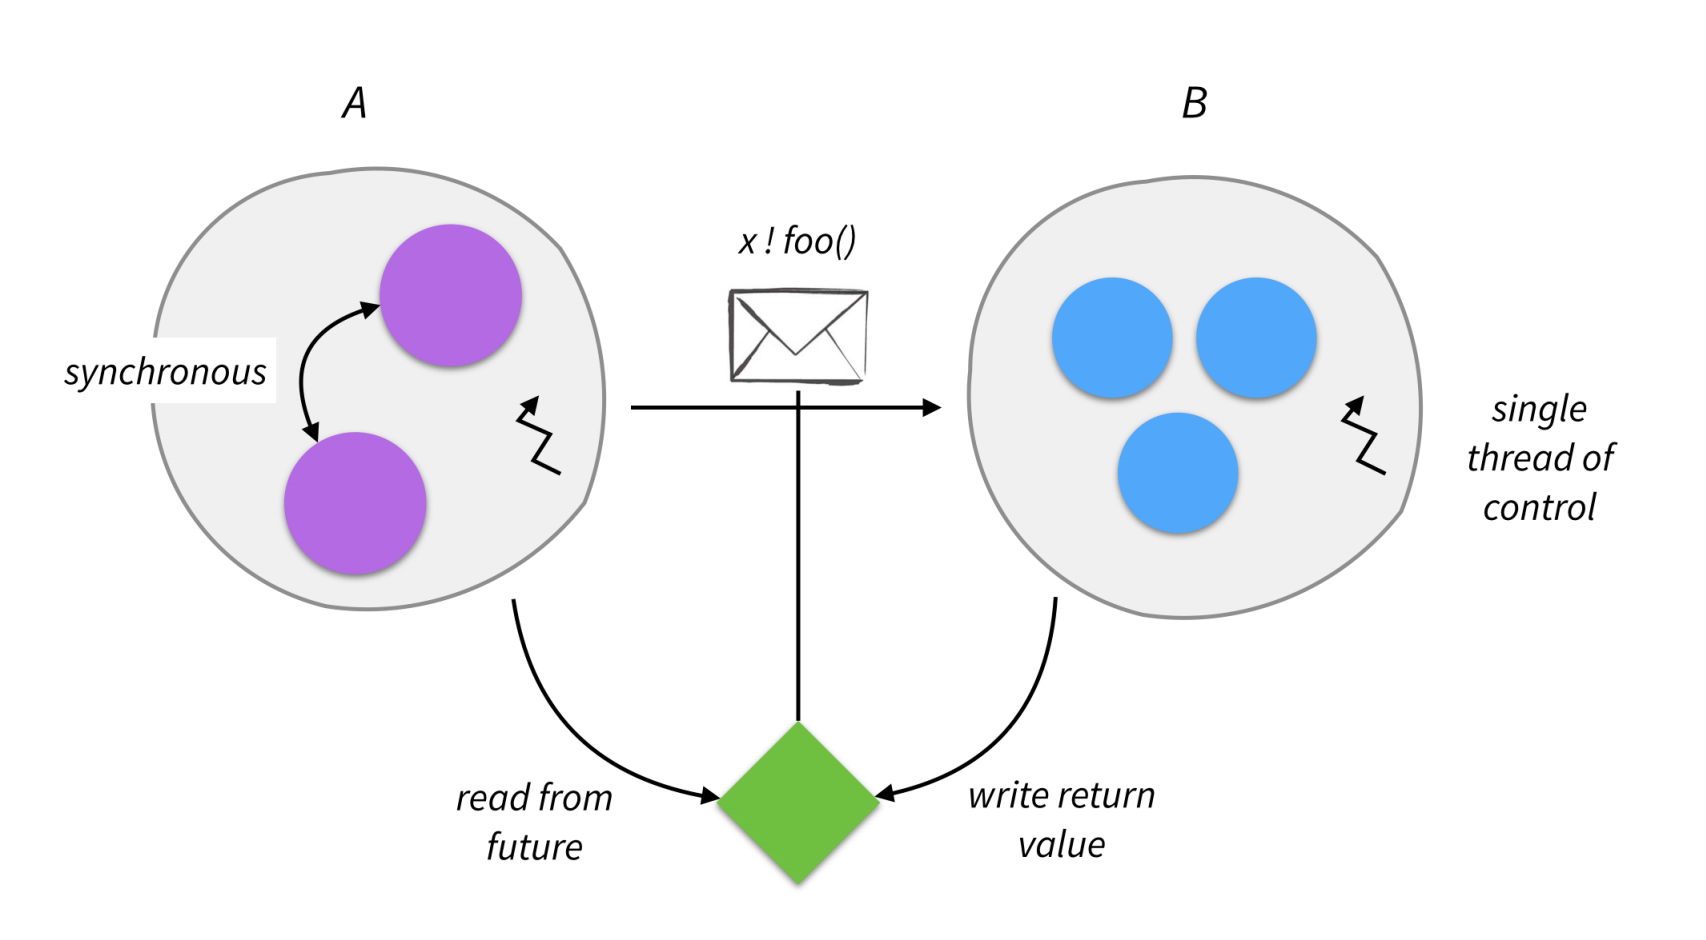
\includegraphics[width=12cm]{images/active-model-figure}
Figure(1): Graphical view of message passing and futures in Encore \citep{encore_paper}.
\end{figure}

\subsection{Kappa - Type System}
Kappa is the name of the type system that is implemented in Encore, it is based previously studies of reference capabilities for concurrency control \citep{kappa}\citep{lolcat}. Kappa Ensures that no data races occur without locks by assigning a mode to all passive class declaration. These modes determine how the object later can be shared during the program runtime. Data-races can normally be hard to debug but in Encore the compiler will catch those errors. \\ 

Local classes can aliased but not shared between active objects. Read classes is safe to share because it can only hold constant fields and can't be mutated. Linear classes can not be aliased and can only be share if it is consumed with the consume keyword, if an linear object is consumed the ownership of that object is transferred to the new instance. At all times there are only one usable reference to a linear object \citep{encore}. 

\subsection{Encore Syntax}
\begin{lstlisting}
active class Main
  def main() : unit
    print("Hello, world!")
  end
end
\end{lstlisting}
The classic Hello World program in Encore, all Encore programs consist of at least one active class and a main method.
\\\\
Encore Syntax is a mix with both functionally and classic imperative styles with inspiration from Languages like Haskel, Scala and Erlang. Calls to method of active objects use the (!) Bang operation, these calls are asynchronous. The future returned can be accessed by using the get keyword. Synchronous calls to passive classes use the classic (.) operation \citep{encore_paper}. In Encore Null or nil does not exist, instead it use maybe types. When declaring a maybe int it can either be of type int or Nothing, patter matching can be used to extract values from maybe types. 

\begin{lstlisting}
active class Main
    def main() : unit
        var person = new Person("Josef", 22)
        var modifier = new NameModifier()
        var fut = modifier ! changeName(consume person, "Dave")
        person = get(fut)
    end
end

linear class Person
    var name : String
    var age : int
    def init(name:String, age:int)
        this.name = name
        this.age = age
    end
end

active class NameModifier
    def changeName(person:Person, name:String) : Person 
        person.name = name
    end
end
\end{lstlisting}
This program showcase both active and passive classes, sharing of mutable data, futures and method calls. The program can be compiled and run by using 'encorec -r program\_name' command. \\

\section{Data Parallel Model}
In the Data Parallel Model focus is on preforming operations on a data sets that are structured as an array or a cube. Tasks are preformed on the data and each task work on a different part of the data-structure. Data parallelism can easily be applied when calculations don’t need result from other parts of the data set. If then the data set is big the program should increase in performance if many cores is provided \citep{paralell-computing}.

\section{MapReduce Framework}
MapReduce is a programming model that have been implemented in many different programming languages. It’s for problems that can be run in parallel, have large amount of input data and have access to big numbers of computational nodes. The programmer only needs to prepare the input and write two functions. One Map function and one Reduce function, the algorithm will provide the rest. The three main steps of the algorithm is “Map”, “Shuffle” and the “Reduce” stage. In the Map stage every node applies the users map function to the local data. The shuffle step then redistribute the data depending on the output from the map step. The Reduce step then finally process each group of data and outputs a result \citep{mapreduce}.
